\chapter{Fitting and Interpreting GLMs {\color{red} DRAFT} \label{chapter:fitglm}}

We've seen the definition of GLMs and a lot of the math behind them in Chapter~\ref{chapter:glms}. Now it's time to talk about how to fit them in R and/or Python and how to interpret the model output. 

%%%%%%%%%%%%%%%%%%%%%%%%%%%%%%%%%%%%%%%%%%%%%%%%%%%%%%%%%%%%%%%%%%%%%%%%%%%%%%%

\section*{Example: Linear Regression}

The following data come from an early study that examined the possible link between air pollution and mortality. The authors examined 60 cities throughout the United States and recorded the following data:

\begin{center}
\texttt{
\begin{tabular}{ll}
\toprule
MORT & Total age-adjusted mortality from all causes, \\
& in deaths per 100,000 population \\
PRECIP & Mean annual precipitation (in inches) \\
EDUC & Median number of school years completed \\
& for persons of age 25 years or older \\
NONWHITE & Percentage of the 1960 population that is nonwhite \\
NOX & Relative pollution potential of oxides of nitrogen \\
SO2 & Relative pollution potential of sulfur dioxide \\
\bottomrule
\end{tabular}
}
\end{center}

Note: ``Relative pollution potential'' refers to the product of the tons emitted per day per square kilometer and a factor correcting the SMSA dimensions and exposure.

We want to predict the value of \texttt{MORT} ($y$) using the predictors \texttt{PRECIP, EDUC, NONWHITE, NOX,} and \verb|SO2| ($x_1, x_2, x_3, x_4$ and $x_5$). 

\subsection*{Fitting in R}

To fit the model in R, you would use the \texttt{lm} command, which fits a linear regression model using ordinary least squares. Basically this package finds the analytical solution that maximizes the likelihood for linear regression, so it is taking advantage of the fact that such an analytical solution exists.

\noindent The commands for fitting the model are:
{\small
\begin{verbatim}
d <- read.csv("lecture-2-data/linear-small-cities-data.csv")
m <- lm(MORT ~ PRECIP + EDUC + NONWHITE + NOX + SO2, data = d)
summary(m)
\end{verbatim}
}

\noindent The output of that last \texttt{summary} command is:

{\small
\begin{verbatim}
Call:
lm(formula = MORT ~ PRECIP + EDUC + NONWHITE + NOX + SO2, data = d)

Residuals:
   Min     1Q Median     3Q    Max 
-91.38 -18.97  -3.56  16.00  91.83 

Coefficients:
             Estimate Std. Error t value Pr(>|t|)    
(Intercept) 995.63646   91.64099  10.865 3.35e-15 ***
PRECIP        1.40734    0.68914   2.042 0.046032 *  
EDUC        -14.80139    7.02747  -2.106 0.039849 *  
NONWHITE      3.19909    0.62231   5.141 3.89e-06 ***
NOX          -0.10797    0.13502  -0.800 0.427426    
SO2           0.35518    0.09096   3.905 0.000264 ***
---
Signif. codes:  0 ?***? 0.001 ?**? 0.01 ?*? 0.05 ?.? 0.1 ? ? 1

Residual standard error: 37.09 on 54 degrees of freedom
Multiple R-squared:  0.6746,	Adjusted R-squared:  0.6444 
F-statistic: 22.39 on 5 and 54 DF,  p-value: 4.407e-12
\end{verbatim}
}

\subsection*{Fitting in Python}

In Python, the \texttt{sklearn} package has a linear regression model. You fit it using the following commands:

{\small
\begin{verbatim}
from sklearn import linear_model
import pandas as pd

d = pd.read_csv("lecture-2-data/linear-small-cities-data.csv")
y = d[["MORT"]]
X = d[["PRECIP", "EDUC", "NONWHITE", "NOX", "SO2"]]
lr = linear_model.LinearRegression()
lr.fit(X, y)
lr.coef_
\end{verbatim}
}
\noindent The output is somewhat less thrilling than R's:
{\small
\begin{verbatim}
array([[  1.40734044, -14.80139073,   3.19909076,  -0.10796976,
          0.35517618]])
\end{verbatim}
}
\noindent but you will notice that the coefficients are identical to those found by R. There are just a lot fewer model diagnostics, etc. If you want something that more closely approximates R's output, you can use the \texttt{statsmodels} package in Python. The commands there are:

{\small
\begin{verbatim}
import statsmodels.api as sm

d = pd.read_csv("lecture-2-data/linear-small-cities-data.csv")
y = d[["MORT"]]
X = d[["PRECIP", "EDUC", "NONWHITE", "NOX", "SO2"]]
X = sm.add_constant(X)  # <- manually add the intercept
lr = sm.OLS(y, X)
results = lr.fit()
print(results.summary())
\end{verbatim}
}
\noindent and the output looks like this:
{\small
\begin{verbatim}
                            OLS Regression Results                            
==============================================================================
Dep. Variable:                   MORT   R-squared:                       0.675
Model:                            OLS   Adj. R-squared:                  0.644
Method:                 Least Squares   F-statistic:                     22.39
Date:                Tue, 17 Oct 2017   Prob (F-statistic):           4.41e-12
Time:                        22:37:41   Log-Likelihood:                -298.78
No. Observations:                  60   AIC:                             609.6
Df Residuals:                      54   BIC:                             622.1
Df Model:                           5                                         
Covariance Type:            nonrobust                                         
==============================================================================
                 coef    std err          t      P>|t|      [0.025      0.975]
------------------------------------------------------------------------------
const        995.6365     91.641     10.865      0.000     811.907    1179.366
PRECIP         1.4073      0.689      2.042      0.046       0.026       2.789
EDUC         -14.8014      7.027     -2.106      0.040     -28.891      -0.712
NONWHITE       3.1991      0.622      5.141      0.000       1.951       4.447
NOX           -0.1080      0.135     -0.800      0.427      -0.379       0.163
SO2            0.3552      0.091      3.905      0.000       0.173       0.538
==============================================================================
Omnibus:                        2.519   Durbin-Watson:                   1.375
Prob(Omnibus):                  0.284   Jarque-Bera (JB):                1.861
Skew:                           0.136   Prob(JB):                        0.394
Kurtosis:                       3.819   Cond. No.                     1.79e+03
==============================================================================
\end{verbatim}
}

%%%%%%%%%%%%%%%%%%%%%%%%%%%%%%%%%%%%%%%%%%%%%%%%%%%%%%%%%%%%%%%%%%%%%%%%%%%%%%%

\section*{Example: Logistic Regression}

The goal of this study was to identify risk factors associated with giving birth to a low birth weight baby (a baby weighing less than 2500 grams). Infant mortality rates and birth defect rates are very high for low birth weight babies. A woman's behavior during pregnancy (including diet, smoking habits, and receiving prenatal care) can greatly alter the chances of carrying the baby to term and, consequently, of delivering a baby of normal birth weight.

Data were collected on 189 women, 59 of which had low birth weight babies and 130 of which had normal birth weight babies.

SOURCE: Hosmer and Lemeshow (2000) \emph{Applied Logistic Regression: Second Edition}. Data were collected at Baystate Medical Center, Springfield, Massachusetts during 1986. 

\begin{center}
\texttt{ \small
\begin{tabular}{ll}
\toprule
LOW & Low birth weight (0 = birth weight $\geq$ 2500 g;\\
& 1 = birth weight $< 2500$ g) \\
AGE & Age of mother in years \\
LWT & Mother's weight in pounds at last menstrual period \\
RACE & Race (1 = white, 2 = black, 3 = other) \\
SMOKE & Smoking status during pregnancy (1 = yes, 0 = no) \\
PTL & History of premature labor (0 = none, 1 = one, etc.) \\
HT & History of hypertension (0 = no, 1 = yes) \\
UI & Presence of uterine irritability (0 = no, 1 = yes) \\
FTV & Number of physician visits during the first trimester \\
BWT & Birth weight in grams \\
\bottomrule
\end{tabular}
}
\end{center}

We would like to predict \texttt{LOW} based on all of the other covariates except \texttt{BWT} (why not use \texttt{BWT}?). 

\subsection*{Fitting in R}

To fit in R, we use the \texttt{glm} package, which fits GLMs using a numerical technique called Fisher scoring. The commands are:

{\small
\begin{verbatim}
d <- read.delim("lecture-2-data/logistic-lowbwt-data.tsv")
d$RACE <- as.factor(d$RACE)  # <- ensure RACE is coded as factor, not number
m <- glm(LOW ~ AGE + LWT + RACE + SMOKE + PTL + HT + UI + FTV, 
         family = "binomial", data = d)
summary(m)
\end{verbatim} 

\noindent The output of this model is:

\begin{verbatim}
Call:
glm(formula = LOW ~ AGE + LWT + RACE + SMOKE + PTL + HT + UI + 
    FTV, family = "binomial", data = d)

Deviance Residuals: 
    Min       1Q   Median       3Q      Max  
-1.8946  -0.8212  -0.5316   0.9818   2.2125  

Coefficients:
             Estimate Std. Error z value Pr(>|z|)   
(Intercept)  0.480623   1.196888   0.402  0.68801   
AGE         -0.029549   0.037031  -0.798  0.42489   
LWT         -0.015424   0.006919  -2.229  0.02580 * 
RACE2        1.272260   0.527357   2.413  0.01584 * 
RACE3        0.880496   0.440778   1.998  0.04576 * 
SMOKE        0.938846   0.402147   2.335  0.01957 * 
PTL          0.543337   0.345403   1.573  0.11571   
HT           1.863303   0.697533   2.671  0.00756 **
UI           0.767648   0.459318   1.671  0.09467 . 
FTV          0.065302   0.172394   0.379  0.70484   
---
Signif. codes:  0 ?***? 0.001 ?**? 0.01 ?*? 0.05 ?.? 0.1 ? ? 1

(Dispersion parameter for binomial family taken to be 1)

    Null deviance: 234.67  on 188  degrees of freedom
Residual deviance: 201.28  on 179  degrees of freedom
AIC: 221.28

Number of Fisher Scoring iterations: 4
\end{verbatim}
}

\subsection*{Fitting in Python}

You can use \texttt{scikit-learn} to fit logistic regression models as well. The commands are not nearly as straightforward:

{\small
\begin{verbatim}
from sklearn import linear_model, preprocessing
import pandas as pd

d = pd.read_table("lecture-2-data/logistic-lowbwt-data.tsv", sep="\t")
y = d[["LOW"]].values.ravel()
X = d[["AGE", "LWT", "RACE", "SMOKE", "PTL", "HT", "UI", "FTV"]]
X["RACE"] = X["RACE"].astype('category')

race_recoded = pd.get_dummies(X, columns=["RACE"])
X = X[["AGE", "LWT", "SMOKE", "PTL", "HT", "UI", "FTV"]].join(
                    race_recoded.ix[:, 'RACE_2':])
  
lr = linear_model.LogisticRegression(C=100000.0, fit_intercept=True,
          penalty='l2', solver='liblinear', tol=0.00001)
lr.fit(X, y)
lr.coef_
\end{verbatim}
}

\noindent But the end result is the same as what we got earlier in R:

{\small
\begin{verbatim}
array([[-0.02952438, -0.01542876,  0.93984778,  0.54233679,  1.864694  ,
         0.76721899,  0.06538879,  1.27277704,  0.8812321 ]])
\end{verbatim}
}

\noindent where we must notice that the columns are in a different order:

{\small
\begin{verbatim}
array(['AGE', 'LWT', 'SMOKE', 'PTL', 'HT', 'UI', 'FTV', 'RACE_2', 'RACE_3'], 
      dtype=object)
\end{verbatim}
}

\noindent We can also do this in Python using \texttt{statsmodels}. 

{\small
\begin{verbatim}
import statsmodels.api as sm

d = pd.read_table("lecture-2-data/logistic-lowbwt-data.tsv", sep="\t")
y = d[["LOW"]].values.ravel()
X = d[["AGE", "LWT", "RACE", "SMOKE", "PTL", "HT", "UI", "FTV"]]
X["RACE"] = X["RACE"].astype('category')
race_recoded = pd.get_dummies(X, columns=["RACE"])
X = X[["AGE", "LWT", "SMOKE", "PTL", "HT", "UI", "FTV"]].join(
     race_recoded.ix[:, 'RACE_2':])
X = sm.add_constant(X)  # <- manually add the intercept
lr = sm.Logit(y, X)
results = lr.fit()
print(results.summary())
\end{verbatim}
}

\noindent The results look like this:

{\small
\begin{verbatim}
                           Logit Regression Results                           
==============================================================================
Dep. Variable:                      y   No. Observations:                  189
Model:                          Logit   Df Residuals:                      179
Method:                           MLE   Df Model:                            9
Date:                Wed, 18 Oct 2017   Pseudo R-squ.:                  0.1423
Time:                        07:51:27   Log-Likelihood:                -100.64
converged:                       True   LL-Null:                       -117.34
                                        LLR p-value:                 0.0001143
==============================================================================
                 coef    std err          z      P>|z|      [0.025      0.975]
------------------------------------------------------------------------------
const          0.4806      1.197      0.402      0.688      -1.865       2.827
AGE           -0.0295      0.037     -0.798      0.425      -0.102       0.043
LWT           -0.0154      0.007     -2.229      0.026      -0.029      -0.002
SMOKE          0.9388      0.402      2.335      0.020       0.151       1.727
PTL            0.5433      0.345      1.573      0.116      -0.134       1.220
HT             1.8633      0.698      2.671      0.008       0.496       3.230
UI             0.7676      0.459      1.671      0.095      -0.133       1.668
FTV            0.0653      0.172      0.379      0.705      -0.273       0.403
RACE_2         1.2723      0.527      2.412      0.016       0.239       2.306
RACE_3         0.8805      0.441      1.998      0.046       0.017       1.744
==============================================================================
\end{verbatim}
}

%%%%%%%%%%%%%%%%%%%%%%%%%%%%%%%%%%%%%%%%%%%%%%%%%%%%%%%%%%%%%%%%%%%%%%%%%%%%%%%

\section*{Example: Poisson Regression}

These data come from a study of nesting horseshoe crabs. Each of the 173 observed female horseshoe crabs had a male crab resident in her nest. The study investigated factors affecting whether the female crab had any other males, called \emph{satellites}, residing nearby. (Source: Agresti, \emph{Categorical Data Analysis}, Table 4.3. Data courtesy of Jane Brockmann, Zoology Department, University of Florida; study described in \emph{Ethology} \textbf{102}: 1-21, 1996.)

\begin{center}
\texttt{\small
\begin{tabular}{ll}
\toprule
SATELL & Number of satellites \\
COLOR & Color of the female crab \\
& (1 = light medium, 2 = medium, 3 = dark medium, 4 = dark) \\
SPINE & Spine condition \\
& (1 = both good, 2 = one work or broken, 3 = both worn or broken) \\
WIDTH & Carapace width of the female crab (cm) \\
WEIGHT & Weight of the female crab (g) \\
\bottomrule
\end{tabular}
}
\end{center}

\subsection*{Fitting in R}

\noindent To fit in R, we again use the \texttt{glm} package. The commands are:

{\small
\begin{verbatim}
d <- read.table("lecture-2-data/poisson-crab-data.txt", head=TRUE)
m <- glm(satell ~ color + spine + width + weight, family = "poisson", data = d)
summary(m)
\end{verbatim} 
}

\noindent The output of this model is:

{\small
\begin{verbatim}
Call:
glm(formula = satell ~ color + spine + width + weight, family = "poisson", 
    data = d)

Deviance Residuals: 
    Min       1Q   Median       3Q      Max  
-3.0126  -1.8846  -0.5406   0.9448   4.9602  

Coefficients:
              Estimate Std. Error z value Pr(>|z|)   
(Intercept) -0.3435447  0.9684204  -0.355  0.72278   
color       -0.1849325  0.0665236  -2.780  0.00544 **
spine        0.0399764  0.0568062   0.704  0.48160   
width        0.0275251  0.0479425   0.574  0.56588   
weight       0.0004725  0.0001649   2.865  0.00417 **
---
Signif. codes:  0 ?***? 0.001 ?**? 0.01 ?*? 0.05 ?.? 0.1 ? ? 1

(Dispersion parameter for poisson family taken to be 1)

    Null deviance: 632.79  on 172  degrees of freedom
Residual deviance: 551.85  on 168  degrees of freedom
AIC: 917.15

Number of Fisher Scoring iterations: 6
\end{verbatim}
}

\subsection*{Fitting in Python}

\noindent Right now \texttt{scikit-learn} does not allow you to use Poisson regression, but it looks like they're working on it:

\begin{center}
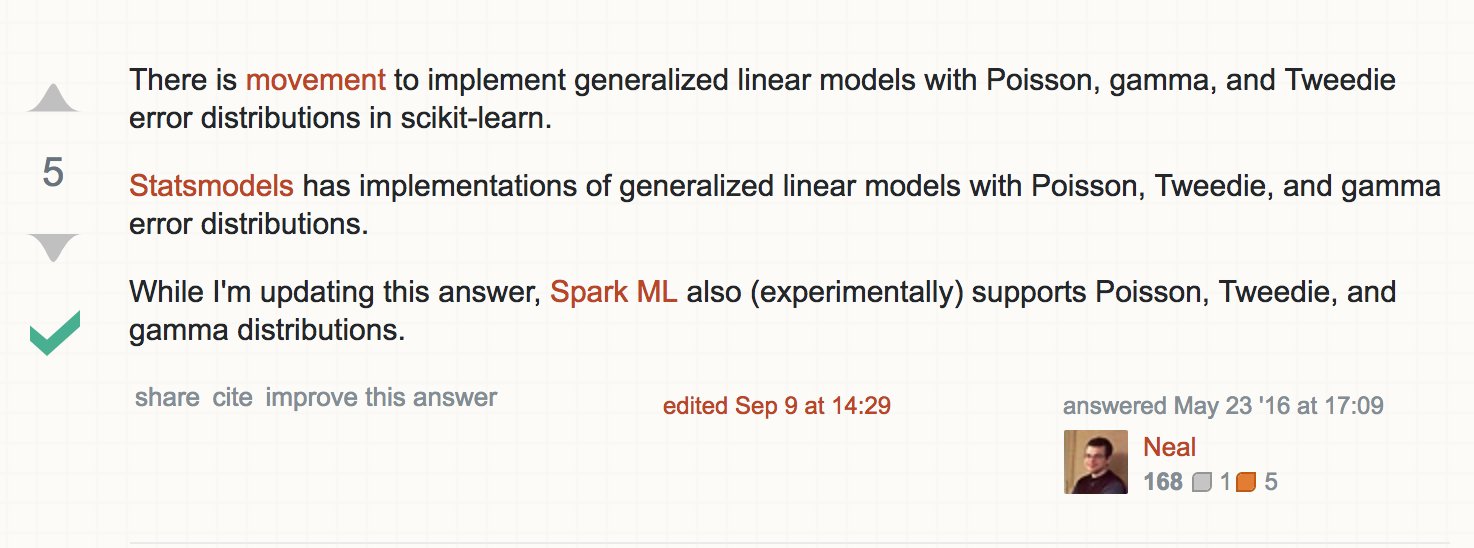
\includegraphics[width=\textwidth]{img/l02-stack-overflow-poisson-reg.png}
\end{center}

\noindent For now I would suggest using \texttt{statsmodels}. Here's how you'd do Poisson regression using that package:

{\small
\begin{verbatim}
import statsmodels.api as sm

d = pd.read_table("lecture-2-data/poisson-crab-data.txt", 
                  sep=r"\s*", engine="python")
y = d[["satell"]].values.ravel()
X = d[["color", "spine", "width", "weight"]]
X = sm.add_constant(X)  # <- manually add the intercept
lr = sm.Poisson(y, X)
results = lr.fit()
print(results.summary())
\end{verbatim}
}

\noindent And here's the output:

{\small
\begin{verbatim}
                          Poisson Regression Results                          
==============================================================================
Dep. Variable:                      y   No. Observations:                  173
Model:                        Poisson   Df Residuals:                      168
Method:                           MLE   Df Model:                            4
Date:                Wed, 18 Oct 2017   Pseudo R-squ.:                 0.08191
Time:                        07:50:24   Log-Likelihood:                -453.58
converged:                       True   LL-Null:                       -494.04
                                        LLR p-value:                 1.102e-16
==============================================================================
                 coef    std err          z      P>|z|      [0.025      0.975]
------------------------------------------------------------------------------
const         -0.3435      0.968     -0.355      0.723      -2.242       1.555
color         -0.1849      0.067     -2.780      0.005      -0.315      -0.055
spine          0.0400      0.057      0.704      0.482      -0.071       0.151
width          0.0275      0.048      0.574      0.566      -0.066       0.121
weight         0.0005      0.000      2.865      0.004       0.000       0.001
==============================================================================
\end{verbatim}
}
